\documentclass[11pt, a4paper]{article}
\usepackage{amsmath, amsthm, amssymb}
\usepackage{stmaryrd}
\usepackage{geometry}
\usepackage[hidelinks]{hyperref}
\usepackage{microtype}
\usepackage{booktabs}
\usepackage{xcolor}
\usepackage{tikz}
\usepackage{parskip}

% parskip is reset to 0 inside \parbox/minipage (the coloured boxes);
% restore it so paragraphs are separated by blank lines everywhere.
\makeatletter
\g@addto@macro\@arrayparboxrestore{\setlength{\parskip}{.5\baselineskip}}
\makeatother

\geometry{margin=2.5cm}

\theoremstyle{definition}
\newtheorem{definition}{Definition}[section]
\newtheorem{example}[definition]{Example}
\newtheorem{remark}[definition]{Remark}
\theoremstyle{plain}
\newtheorem{proposition}[definition]{Proposition}
\newtheorem{theorem}[definition]{Theorem}
\newtheorem{exercise}[definition]{Exercise}

\newcommand{\droot}{\mathsf{root}}
\newcommand{\dsub}{\mathbin{\downarrow}}
\newcommand{\dshift}{\mathbin{\oplus}}

\title{Coloured Graphs as Directed Containers\\[0.4em]
\large with an application to INSTINCT}
\author{Robin Langer}
\date{July 2026}

\begin{document}
\maketitle

% ─────────────────────────────────────────────────────────────────────────────
\section{Containers and Types}
% ─────────────────────────────────────────────────────────────────────────────

\noindent\colorbox{gray!15}{\parbox{\dimexpr\linewidth-2\fboxsep}{%
\begin{definition}
A \emph{container} is a pair $\psi = (S, P)$ where $S$ is a set of \emph{shapes} and
\[
  P : S \to \mathbf{Set}(A)
\]
is a family of \emph{positions}, where $\mathbf{Set}(A)$ is the set of all
subsets of $A$ for some universal set $A$.

For any given shape $s$, think of $P(s) \subseteq A$ as a set of
``slots'' where you can put data.  We don't actually have any data
yet.  That will come later when we do extensions of containers.
\end{definition}%
}}

\begin{example}\label{ex:list}
A \emph{list} is described by
the container $L$ with shapes $S_L = \mathbb{N}$ (the length) and positions
\[
  P_L : \mathbb{N} \to \mathbf{Set}(\mathbb{N}), \qquad
  P_L(n) = \{1, 2, \ldots, n\}.
\]
Note that this container represents lists of
any length.  But it doesn't yet contain any data.  Think of it as
the type of a list.
\end{example}

\begin{example}\label{ex:tree}
Encode a vertex of a binary tree as a word in
$\{\mathrm{L}, \mathrm{R}\}^*$ --- the directions taken from the
root.  A finite set $t \subseteq \{\mathrm{L}, \mathrm{R}\}^*$ is a
\emph{valid tree shape} when it is
\emph{prefix-closed}.  That is, every prefix $w'$ of a word
$w \in t$ is also in $t$.  The empty word (the root) belongs to every nonempty
tree.  Let $\mathrm{Tree}$ be the set of all valid tree shapes, and let
\[
  T = (\mathrm{Tree}, Q), \qquad
  Q : \mathrm{Tree} \to \mathbf{Set}(\{\mathrm{L},\mathrm{R}\}^*),
  \qquad Q(t) = t,
\]
We denote by $V(t)$ the number of vertices of $t$.

If you already have an image in your mind of what a tree looks
like, imagine that each vertex of the tree is a ``slot'' where we
could add data.  As before, we don't have any data yet.  This is
just the type of a tree.
\end{example}

\noindent\colorbox{blue!10}{\parbox{\dimexpr\linewidth-2\fboxsep}{%
\begin{remark}\label{rem:dependent-types}
For any container $(S, P)$ and any $s \in S$ we may associate a
\emph{dependent type}:
\[
  s : S \vdash P(s) : \texttt{Type}.
\]
Very few programming languages support dependent types, the exceptions
being Lean, Agda, Idris, and Coq.

We haven't actually said what a \texttt{Type} is yet.  But we will.
\end{remark}%
}}

\begin{example}\label{ex:haskell}
Haskell does not support dependent types.  In Haskell the list
and the tree are defined by
\begin{center}
\colorbox{gray!15}{\begin{minipage}{0.85\linewidth}
\ttfamily
data List a = Nil | Cons a (List a)\\
data Tree a = Leaf | Node (Tree a) a (Tree a)
\end{minipage}}
\end{center}
A list of \texttt{a}s is either empty, or an element together with
another list.  A tree is either a leaf, or a node carrying an
element and two subtrees.  The types are defined recursively.

In Haskell we cannot define a
list of a specific length or a tree of a specific shape.  The best
we can do is a run-time check.
\begin{center}
\colorbox{gray!15}{\begin{minipage}{0.75\linewidth}
\ttfamily
mkListOfLength :: Int -> [a] -> Maybe [a]\\
mkListOfLength n xs\\
\hspace*{1.5em}| length xs == n\hspace*{0.5em}= Just xs\\
\hspace*{1.5em}| otherwise\hspace*{3.5em}= Nothing
\end{minipage}}
\end{center}
\end{example}

\begin{example}\label{rem:c-pointers}
Recursion in C is
implemented using pointers.
A position is an \emph{address}.  A labelling of the positions with
data is the \emph{memory contents}.

What is the type of a \emph{linked list}?  In C one writes
\begin{center}
\colorbox{gray!15}{\begin{minipage}{0.75\linewidth}
\ttfamily
typedef struct Node *List;\\[4pt]
struct Node \{\\
\hspace*{1.5em}int data;\\
\hspace*{1.5em}struct Node *next;\\
\};
\end{minipage}}
\end{center}
The list is given the type of a pointer to its first node.
In C, every pointer type is either a
valid address or \texttt{NULL}.  Unfolding it, a node is a
datum together with either another node or \texttt{NULL}, so a
linked list is either empty, or a head and a tail.  C cannot express the recursion directly, so it
smuggles it in with pointers.

Likewise a binary tree.
\begin{center}
\colorbox{gray!15}{\begin{minipage}{0.75\linewidth}
\ttfamily
typedef struct TNode *Tree;\\[4pt]
struct TNode \{\\
\hspace*{1.5em}int data;\\
\hspace*{1.5em}struct TNode *left;\\
\hspace*{1.5em}struct TNode *right;\\
\};
\end{minipage}}
\end{center}
A tree is a pointer to its root, the empty tree is \texttt{NULL},
and each node now carries two pointers --- one slot for each
child.

What does C check?  Pointer types are checked at compile time, a
pointer to one type of struct cannot point to a struct of a
different type, and within a struct only the declared fields can
be named.

What does C not check?
\begin{itemize}
\item Bounds --- trying to access the 7th element of a list of
  length 5 (the buffer overflow).
\item Nullness --- following a pointer that points to
  \texttt{NULL}.
\item Dangling pointers --- for example, after removing
  an element from the end of a list you might forget to point the
  previous pointer to \texttt{NULL}.
\end{itemize}

This is ugly, which is the reason why people prefer to
program in higher level languages.
\end{example}

\noindent\colorbox{blue!10}{\parbox{\dimexpr\linewidth-2\fboxsep}{%
\begin{example}\label{ex:lean-dependent}
One language that does support dependent types is Lean.
For example, we can define a vector of length \texttt{n} containing
entries from \texttt{a} as follows:
\begin{center}
\colorbox{gray!15}{\begin{minipage}{0.85\linewidth}
\ttfamily
inductive Vec (a : Type) : Nat -> Type where\\
\hspace*{1.5em}| nil\hspace*{1.5em}: Vec a 0\\
\hspace*{1.5em}| cons : a -> Vec a n -> Vec a (n + 1)
\end{minipage}}
\end{center}
\texttt{Vec a n} is the type of a list of length \texttt{n}.  Note that it
doesn't actually have any data yet.  It is a type.

Note that \texttt{(Vec a)} is a \emph{type constructor}, of signature
\begin{center}
\colorbox{gray!15}{\begin{minipage}{0.85\linewidth}
\ttfamily
(Vec a) : Nat -> Type
\end{minipage}}
\end{center}
The type constructor depends on a \emph{value} \texttt{n} of type
\texttt{Nat}, and returns a \texttt{Type}.

A function
from values to types is called a \emph{dependent family} --- it is the
same kind of object as the position family
$P_L : \mathbb{N} \to \mathbf{Set}(\mathbb{N})$ that we saw for lists.

$P_L(n) = \{1, 2, \ldots, n\}$ is \texttt{Vec a n}.

To construct a vector of length 3 in Lean we write:
\begin{center}
\colorbox{gray!15}{\begin{minipage}{0.85\linewidth}
\ttfamily
def v : Vec Int 3 := cons 1 (cons 2 (cons 3 nil))
\end{minipage}}
\end{center}
The list now contains data, \texttt{v} is a value of type
\texttt{Vec Int 3}.
This is a recursive construction.  The length is tracked in the type at every step.
The way we put data into containers is different.  We don't need
recursion, instead we just ``slot it in''.  This is one of the great
powers of container theory.

\medskip
\noindent
Why would anybody do this?  The idea is to catch a vector length mis-match
at compile time rather than run time.

Dependent types come at a price.  If types contain values, then deciding
whether two types are equal requires deciding whether two values are
equal, so the type checker must \emph{execute code} at compile time.

\medskip
\noindent
If types contain values, then types contain \emph{computations}.
For example:
\begin{center}
\colorbox{gray!15}{\begin{minipage}{0.85\linewidth}
\ttfamily
Vec a (n + m) = Vec a (m + n)
\end{minipage}}
\end{center}
describe vectors of the same length, but we must prove they are
the same type.  This is extremely tedious and painful.
\end{example}%
}}

\section{Sums and products of containers}

\noindent\colorbox{gray!15}{\parbox{\dimexpr\linewidth-2\fboxsep}{%
\begin{definition}\label{def:sum-functions}
The \emph{categorical sum} of two sets $A$ and $B$ is their
\emph{disjoint union} $A \sqcup B$.
\[
  \mathrm{left} : A \to A \sqcup B,
  \qquad
  \mathrm{right} : B \to A \sqcup B.
\]
The sum extends to \emph{functions}.  Given $f : A \to C$ and
$g : B \to D$, their sum
\[
  f \sqcup g : A \sqcup B \to C \sqcup D
\]
is defined by the unique function
making the two squares commute.
\[
\begin{array}{ccc}
  A & \xrightarrow{\;\mathrm{left}\;} & A \sqcup B\\[2pt]
  \big\downarrow{\scriptstyle f} & & \big\downarrow{\scriptstyle f \sqcup g}\\[2pt]
  C & \xrightarrow{\;\mathrm{left}\;} & C \sqcup D
\end{array}
\qquad\qquad
\begin{array}{ccc}
  B & \xrightarrow{\;\mathrm{right}\;} & A \sqcup B\\[2pt]
  \big\downarrow{\scriptstyle g} & & \big\downarrow{\scriptstyle f \sqcup g}\\[2pt]
  D & \xrightarrow{\;\mathrm{right}\;} & C \sqcup D
\end{array}
\]
\end{definition}%
}}

\medskip

\noindent\colorbox{gray!15}{\parbox{\dimexpr\linewidth-2\fboxsep}{%
\begin{definition}\label{def:product-functions}
The \emph{categorical product} of two sets $A$ and $B$ is
their \emph{cartesian product} $A \times B$.  It comes
with the two projections
\[
  \pi_1 : A \times B \to A,
  \qquad
  \pi_2 : A \times B \to B.
\]
The product extends to \emph{functions}.  Given $f : A \to C$ and
$g : B \to D$, their product
\[
  f \times g : A \times B \to C \times D
\]
is
the unique function making the two squares commute.
\[
\begin{array}{ccc}
  A \times B & \xrightarrow{\;\pi_1\;} & A\\[2pt]
  \big\downarrow{\scriptstyle f \times g} & & \big\downarrow{\scriptstyle f}\\[2pt]
  C \times D & \xrightarrow{\;\pi_1\;} & C
\end{array}
\qquad\qquad
\begin{array}{ccc}
  A \times B & \xrightarrow{\;\pi_2\;} & B\\[2pt]
  \big\downarrow{\scriptstyle f \times g} & & \big\downarrow{\scriptstyle g}\\[2pt]
  C \times D & \xrightarrow{\;\pi_2\;} & D
\end{array}
\]
\end{definition}%
}}

\medskip
\noindent
Sums and products can be defined for any category and they are
dual.  Both sum and product ``lift'' naturally to containers.

\medskip
\noindent\colorbox{gray!15}{\parbox{\dimexpr\linewidth-2\fboxsep}{%
\begin{definition}\label{def:sum}
Suppose that we have two containers $\psi = (S, P)$ with
$P : S \to \mathbf{Set}(A)$ and $\varphi = (T, Q)$ with
$Q : T \to \mathbf{Set}(B)$.  Their \emph{sum}
$\psi + \varphi$ is the container whose shapes are the disjoint union
$S \sqcup T$ and whose positions are
\[
  (P + Q) : S \sqcup T \to \mathbf{Set}(A \sqcup B), \qquad
  (P + Q)(s) =
  \begin{cases}
    P(s) & \text{if } s \in S,\\
    Q(s) & \text{if } s \in T.
  \end{cases}
\]
The \emph{product} $\psi \times \varphi$ is the container whose
shapes are the pairs $S \times T$ and whose positions are the
disjoint union
\[
  (P \times Q) : S \times T \to \mathbf{Set}(A \sqcup B),
  \qquad
  (P \times Q)(s, t) = P(s) \sqcup Q(t).
\]
\end{definition}%
}}

\begin{example}\label{ex:list-sum}
Recall the list container $L = (\mathbb{N}, P_L)$ with
$P_L : \mathbb{N} \to \mathbf{Set}(\mathbb{N})$,
$P_L(n) = \{1, 2, \ldots, n\}$.  Note that
\[
  \mathbb{N} = \{1\} \cup \{2\} \cup \{3\} \cup \cdots
\]
so the shapes decompose as the disjoint union of the singletons
$S_k = \{k\}$.  Define a family of individual shape containers.  Let
$P_k : \{k\} \to \mathbf{Set}(\mathbb{N})$ with
$P_k(k) = \{1, 2, \ldots, k\}$, and set $L_k = (S_k, P_k)$.  Then
\[
  L = L_1 + L_2 + L_3 + \cdots
\]
\noindent\colorbox{green!10}{\parbox{\dimexpr\linewidth-2\fboxsep}{%
Each $L_k$ is a dependent type --- it is \texttt{Vec a k}, whose
type depends on the value $k$ --- but the sum $L$ is not.  It is
the ordinary type \texttt{List a}, which we can have in Haskell.%
}}
\end{example}

\begin{example}\label{ex:tree-sum}
Recall the tree container $T = (\mathrm{Tree}, Q)$ of
Example~\ref{ex:tree}, with $Q(t) = t$.  Now $\mathrm{Tree}$
decomposes as
\[
  \mathrm{Tree} = \bigcup_{t \,\in\, \mathrm{Tree}} \{t\},
\]
and for each $t$ we have the individual shape container
$T_t = (\{t\}, Q_t)$ with $Q_t(t) = t$.  So
\[
  T = \sum_{t \,\in\, \mathrm{Tree}} T_t,
\]
\noindent\colorbox{green!10}{\parbox{\dimexpr\linewidth-2\fboxsep}{%
Again each $T_t$ is a dependent type --- the type of trees of valid tree word
exactly $t$, which depends on the value $t$ --- but the sum $T$ is
not.  It is the ordinary type \texttt{Tree a}, which we can have in
Haskell.%
}}
\end{example}

\begin{center}
\colorbox{blue!10}{\parbox{0.9\linewidth}{\centering
Every container is the sum of its individual shape subcontainers.
$\psi = \sum_{s \in S} (\{s\}, P_s)$.}}
\end{center}

\section{Container Morphisms}

\noindent\colorbox{gray!15}{\parbox{\dimexpr\linewidth-2\fboxsep}{%
\begin{definition}\label{def:morphism}
Suppose that we have two containers $\psi = (S, P)$ with
\[
  P : S \to \mathbf{Set}(A)
\]
and $\varphi = (T, Q)$ with
\[
  Q : T \to \mathbf{Set}(A).
\]
They must have the same set of possible positions $A$.
A \emph{morphism} of containers $(u, g) : \psi \to \varphi$ is a map
from the shapes $S$ to the shapes $T$
\[
  u : S \to T
\]
together with a family of arrows, one for each shape $s \in S$,
pointing in the \emph{opposite} direction:
\[
  g_s : Q(u(s)) \mapsto P(s).
\]
The new positions of $T$ can only come from the old positions of
$S$.  This is because new data cannot be created.  The arrow points
backwards to tell you where the data in $t \in T$ came from.
\end{definition}%
}}

\begin{example}\label{ex:reverse}
$\mathrm{reverse}$ is the morphism $L \to L$ of the list container with
\[
  u : n \mapsto n
  \qquad\text{and}\qquad
  g_n : k \mapsto (n + 1 - k).
\]
This says that the new position $k$ came from the old position
$(n + 1 - k)$.
\end{example}

\begin{example}\label{ex:dup}
Let $\mathrm{dup} : L \to L$ be the operation sending the list
$[a, b, c]$ to $[a, a, b, b, c, c]$.  As a container morphism the
shape arrow doubles the length,
\[
  u : n \mapsto 2n,
\]
and the positions arrow sends each new position back to the old
position it copies its data from,
\[
  g_n : (2k - 1) \mapsto k
  \qquad\text{and}\qquad
  g_n : 2k \mapsto k.
\]
This tells you that both the new positions $3$ and $4$ came from the old
position $2$.
\end{example}

\begin{example}\label{ex:tail}
Let $\mathrm{tail} : L \to L$ be the operation sending the list
$[a, b, c, d]$ to $[b, c, d]$.  As a container morphism the shape arrow
decreases the length by one,
\[
  u : n \mapsto n - 1,
\]
and the positions arrow is
\[
  g_n : k \mapsto (k + 1).
\]
This says that the new position $k$ came from the old position
$(k+1)$.
\end{example}

\noindent\colorbox{gray!15}{\parbox{\dimexpr\linewidth-2\fboxsep}{%
\begin{theorem}\label{thm:cont-category}
Containers and container morphisms form a category $\mathbf{Cont}$.
The identity morphism on $\psi = (S, P)$ is
\[
  \mathrm{id}_\psi = \bigl(\mathrm{id}_S,\ (\mathrm{id}_{P(s)})_{s \in S}\bigr),
\]
where for each $s \in S$, the map $\mathrm{id}_{P(s)}$ is the
identity function.  Composition is given by:
\[
  (v, h) \circ (u, g)
  = \bigl(v \circ u,\ (g_s \circ h_{u(s)})_{s \in S}\bigr).
\]
The shape maps compose \emph{forwards},
\[
\begin{array}{ccccc}
  S & \xrightarrow{\;u\;} & T & \xrightarrow{\;v\;} & \tilde{S}
\end{array}
\]
while the position arrows compose \emph{backwards}
\[
\begin{array}{ccccc}
  P(s) & \xleftarrow{\;g_s\;} & Q(u(s))
       & \xleftarrow{\;h_{u(s)}\;} & \tilde{P}(v(u(s))).
\end{array}
\]
Remember that we can't create new data, so the position arrows tell
us where the data came from.  The data doesn't live in $T$, it
lives in $Q(t)$ for some $t \in T$.
The composite $g_s \circ h_{u(s)}$ only has the right
type because the arrow on positions points backwards.
\end{theorem}%
}}

\medskip

\noindent
Associativity and the identity laws are inherited from ordinary
function composition.

\begin{remark}\label{rem:functions-as-morphisms}
Every container morphism $f : A \to B$ can be thought of as a
function of type $A \to B$, but not every function of type
$A \to B$ is a container morphism.

For example, permuting a list is a container morphism but sorting
a list is not.

For simplicity, suppose our language supports only the primitives
\texttt{Int} and \texttt{Bool}, together with their basic
operations.  These are arithmetic, comparison and boolean operations.  None
of these basic operations is a container morphism.

To get a complete language we must also add
\emph{pattern matching} (branching) and \emph{recursion}.  Pattern matching is
case analysis on the constructor of a value.
\end{remark}

\begin{example}\label{ex:product-state}
Consider \emph{tree sort}.  The type of this map is
$\mathrm{sort} : L \times T \to L \times T$.
First we insert the elements from the list into the
tree (according to some criterion), then we read back the elements
from the tree to the list (in a certain order).  The state at each step
is a pair $(L, T)$.  It records what is left to insert, and what has been built so far
--- a list of length $n$ and a search tree $t$ with $k$ vertices.
One step of the algorithm
takes the head of the list and inserts it into the tree:
\[
  \mathrm{insert} : L \times T \to L \times T, \qquad
  (n, t) \;\longmapsto\; (n-1,\; t'),
\]
where $t'$ has one vertex more than $t$, and for the read-back phase
\[
  \mathrm{read} : L \times T \to L \times T, \qquad
  (n, t) \;\longmapsto\; (n+1,\; t''),
\]
where $t''$ has one less vertex than $t$.

For $n = 3$ the full sort algorithm can be expressed as
\[
  \mathrm{read} \circ \mathrm{read} \circ \mathrm{read}
  \circ \mathrm{insert} \circ \mathrm{insert} \circ \mathrm{insert}.
\]
In general, define the iterates recursively.  Set
\[
  \mathrm{insert}_1 = \mathrm{insert},
  \qquad
  \mathrm{insert}_{n+1} = \mathrm{insert} \circ \mathrm{insert}_n,
\]
and likewise
\[
  \mathrm{read}_1 = \mathrm{read},
  \qquad
  \mathrm{read}_{n+1} = \mathrm{read} \circ \mathrm{read}_n.
\]
This allows us to apply insertion sort to a list of any length $n$.
\[
  \mathrm{sort}_n = \mathrm{read}_n \circ \mathrm{insert}_n.
\]

In Haskell:
\begin{center}
\colorbox{gray!15}{\begin{minipage}{0.85\linewidth}
\ttfamily
insert :: Ord a => ([a], Tree a) -> ([a], Tree a)\\
insert (x : xs, t) = (xs, ins x t)\\
\hspace*{1.5em}where\\
\hspace*{3em}ins x Leaf = Node Leaf x Leaf\\
\hspace*{3em}ins x (Node l y r)\\
\hspace*{4.5em}| x <= y\hspace*{1.4em}= Node (ins x l) y r\\
\hspace*{4.5em}| otherwise = Node l y (ins x r)\\[6pt]
read :: ([a], Tree a) -> ([a], Tree a)\\
read (xs, t) = (y : xs, t')\\
\hspace*{1.5em}where\\
\hspace*{3em}(y, t') = removeMax t\\
\hspace*{3em}removeMax (Node l x Leaf) = (x, l)\\
\hspace*{3em}removeMax (Node l x r)\hspace*{1.1em}= (z, Node l x r')\\
\hspace*{4.5em}where (z, r') = removeMax r\\[6pt]
insertN :: Ord a => Int -> ([a], Tree a) -> ([a], Tree a)\\
insertN 1 = insert\\
insertN n = insert . insertN (n - 1)\\[6pt]
readN :: Int -> ([a], Tree a) -> ([a], Tree a)\\
readN 1 = read\\
readN n = read . readN (n - 1)\\[6pt]
sortN :: Ord a => Int -> ([a], Tree a) -> ([a], Tree a)\\
sortN n = readN n . insertN n
\end{minipage}}
\end{center}
This is NOT a container
morphism because it uses comparisons, and pattern matching, and
recursion.
\end{example}

\newpage

\section{Extension of containers and Types}

Now we are ready to put some data into our containers.  In this
section we will ``bootstrap'' the definition of a type.

\noindent\colorbox{gray!15}{\parbox{\dimexpr\linewidth-2\fboxsep}{%
\begin{definition}\label{def:extension}
The \emph{extension} of a container $\psi = (S, P)$ with respect to a set
of labels $X$ (data) is
\[
  C_\psi(X) = \sum_{s:S}\bigl(P(s) \to X\bigr)
            = \bigl\{\langle s, f \rangle : s \in S,\ f : P(s) \to X\bigr\}.
\]
The elements of the extension are pairs $\langle s, f \rangle$.  A shape $s$
together with a labelling $f$ of its positions.  Think of it
as slotting data into the positions of $P(s)$.
For example, if $X = \{\mathrm{True}, \mathrm{False}\}$, then $C_L(X)$ is the
set of lists of type \texttt{Bool} of any length.
\end{definition}%
}}


You can think of the container as ``pure structure'' and the variable $X$ as
a set of labels on that structure.  The labels are data that can be
``slotted in'' to the positions.


\noindent\colorbox{green!10}{\parbox{\dimexpr\linewidth-2\fboxsep}{%
\begin{remark}
A container morphism $(u, g) : \psi \to \varphi$ acts on extensions by
\[
  \langle s, f \rangle \longmapsto \langle u(s),\; f \circ g_s \rangle.
\]
Note again that the arrow $g_s$
points backwards, otherwise you wouldn't be able to compose it with $f$.  We
have $f : P(s) \to X$ and $g_s : \hat{P}(u(s)) \mapsto P(s)$, so
$f \circ g_s : \hat{P}(u(s)) \to X$ is a labelling of the new shape.
\end{remark}%
}}

We are going to ``bootstrap'' the definition of $\texttt{Type}$ by
setting $\texttt{Type}_0 = \{\texttt{Int}, \texttt{Bool}\}$ and then
defining $\texttt{Type}_{k+1}$ recursively in terms of
$\texttt{Type}_k$.

You can think of $\texttt{Type}_3$ as types of
types of types of $\{\texttt{Int}, \texttt{Bool}\}$.

\medskip

Let us define a $2$-indexed container first, we'll work up to the
general definition later.  Start with a ``struct'' containing three
\texttt{Int}s and two \texttt{Bool}s.
\begin{center}
\colorbox{gray!15}{\begin{minipage}{0.85\linewidth}
\ttfamily
struct \{\\
\hspace*{1.5em}int x, y, z;\\
\hspace*{1.5em}bool a, b;\\
\}
\end{minipage}}
\end{center}
As a container this is a single shape $s$ with five slots
\[
  P(s) = \{x, y, z, a, b\}.
\]
The slots come in two ``types''.  We record the type of each slot
with a map into the index set $I = \{\texttt{Int}, \texttt{Bool}\}$,
\[
  r_s : P(s) \to I,
\]
so $r_s(x) = r_s(y) = r_s(z) = \texttt{Int}$ and
$r_s(a) = r_s(b) = \texttt{Bool}$.

\medskip

\noindent\colorbox{gray!15}{\parbox{\dimexpr\linewidth-2\fboxsep}{%
\begin{definition}
Let $I$ be an index set with two elements.  A \emph{$2$-indexed
container over $I$} is a container $\phi = (S, P)$ with, for each
$s \in S$, a map
\[
  r_s : P(s) \to I,
\]
called the \emph{response map}.
\end{definition}%
}}

\medskip

Take $I = \{\texttt{Int}, \texttt{Bool}\}$.  To put data into the
container we choose one data set for each index.
\[
  X_1 = \mathbb{N}
  \qquad\text{for \texttt{Int}, and}\qquad
  X_2 = \{\mathrm{True}, \mathrm{False}\}
  \qquad\text{for \texttt{Bool}.}
\]

\noindent\colorbox{gray!15}{\parbox{\dimexpr\linewidth-2\fboxsep}{%
\begin{definition}
The \emph{extension} of a $2$-indexed container $\phi = (S, P, r)$
over $I$ at the data $(X_1, X_2)$ is
\[
  C_\phi(X_1, X_2) = \sum_{s \in S} \prod_{p \in P(s)} X_{r_s(p)},
\]
where $X_{\texttt{Int}} = X_1$ and $X_{\texttt{Bool}} = X_2$.
\end{definition}%
}}

\medskip

Compare this with the plain extension $C_\psi(X)$ of
Definition~\ref{def:extension}.  There every slot received data from
the \emph{same} set $X$, and a labelling was a function
$f : P(s) \to X$.  Here each slot $p$ has its own data type
$X_{r_s(p)}$.  An \texttt{Int} slot receives a value from $X_1$
and a \texttt{Bool} slot receives a value from $X_2$.

\medskip

For the struct above,
\[
  C_\phi(X_1, X_2)
  = \mathbb{N}^3 \times \{\mathrm{True}, \mathrm{False}\}^2.
\]
An element of the extension slots an actual value into each field.
We now have data in our containers.

\medskip

Now we give the general definition.  The index set $I$ can be any
set, the data is a family $X = (X_i)_{i \in I}$ with one set for
each index, and the shapes are typed as well as the positions.

\noindent\colorbox{gray!15}{\parbox{\dimexpr\linewidth-2\fboxsep}{%
\begin{definition}
Let $I$ be any index set.  An \emph{$I$-indexed container} is a
container $\phi = (S, P)$ with a map $r : S \to I$ typing the
shapes and, for each $s \in S$, a response map $r_s : P(s) \to I$
typing the positions.  Given data $X = (X_i)_{i \in I}$, the
\emph{extension} of $\phi$ at $i \in I$ is obtained by restricting
to $S_i = \{\, s \in S \mid r(s) = i \,\}$, the shapes of type $i$:
\[
  C_\phi{}_{,i}(X)
  = \sum_{s \in S_i} \prod_{p \in P(s)} X_{r_s(p)}.
\]
Think of $I$ as dividing up the positions into different ``types''.
If $p$ is of type $i$ then we choose a value from the data set
$X_i$.
\end{definition}%
}}

\medskip

We can bootstrap the definition of $\texttt{Type}$ using indexed
container extensions.
\begin{align*}
  \texttt{Type}_0 &= \{\texttt{Int}, \texttt{Bool}\},\\
  \texttt{Type}_1 &= \text{indexed container extensions over } \texttt{Type}_0,\\
  \texttt{Type}_2 &= \text{indexed container extensions over } \texttt{Type}_1,\\
  &\;\;\vdots\\
  \texttt{Type}_{k+1} &= \text{indexed container extensions over } \texttt{Type}_k.
\end{align*}

\medskip

\noindent\colorbox{gray!15}{\parbox{\dimexpr\linewidth-2\fboxsep}{%
\begin{definition}\label{def:type-universe}
Define, by induction on the \emph{depth} $k$,
\[
  \texttt{Type}_0 = T = \{\texttt{Int}, \texttt{Bool}\},
\]
and $\texttt{Type}_{k+1}$ to be $\texttt{Type}_k$ together with the
extensions $C_\phi{}_{,x}$ of indexed containers $\phi$ over
$\texttt{Type}_k$.  The universe of types is
\[
  \texttt{Type} = \bigcup_{k \geq 0} \texttt{Type}_k,
\]
and every type has a finite depth.
\end{definition}%
}}

\section{Values from types}

We have defined the types.  To get the \emph{values} we perform one
last container extension.  Take the indexed container over
$I = \texttt{Type}_0$ with shapes $S = \{\texttt{Int},
\texttt{Bool}\}$, where each type has a single slot of that type.  The data is $X_{\texttt{Int}} = \mathbb{N}$ and
$X_{\texttt{Bool}} = \{\mathrm{True}, \mathrm{False}\}$.  The
extension is
\[
  C = \sum_{i \in \texttt{Type}_0} X_i
    = \mathbb{N} \sqcup \{\mathrm{True}, \mathrm{False}\}
    = A,
\]
the set of values.  An element of the extension is a pair of a type
and a value of that type.  This final extension turns a type into a
value.

\medskip

\noindent\colorbox{gray!15}{\parbox{\dimexpr\linewidth-2\fboxsep}{%
Note that $\mathbb{N}$ itself is a container.  Take two
shapes, $\mathrm{zero}$ and $\mathrm{succ}$, where $\mathrm{zero}$
has no slots and $\mathrm{succ}$ has exactly one.
\[
  S = \{\mathrm{zero}, \mathrm{succ}\}, \qquad
  P(\mathrm{zero}) = \varnothing, \qquad
  P(\mathrm{succ}) = \{\ast\}.
\]
A natural number is either $\mathrm{zero}$, or $\mathrm{succ}$ with
another natural number slotted into its single slot.
\[
  3 = \mathrm{succ}(\mathrm{succ}(\mathrm{succ}(\mathrm{zero})))
\]
The naturals are what you get by slotting this container into
itself, over and over.

\medskip

Likewise \texttt{Bool} is a container.  Take two shapes,
$\mathrm{true}$ and $\mathrm{false}$, neither of which has any
slots.
\[
  S = \{\mathrm{true}, \mathrm{false}\},
  \qquad
  P(\mathrm{true}) = P(\mathrm{false}) = \varnothing.
\]
A boolean is a bare shape with nothing slotted in.  There is no
recursion this time.  The two shapes have the same (empty) position
set, so \texttt{Bool} is non-dependent.%
}}

\section{De-categorization}

\noindent\colorbox{blue!10}{\parbox{\dimexpr\linewidth-2\fboxsep}{%
\begin{remark}\label{rem:extension-is-sum}
One can show that for container extensions:
\[
  C_{\psi + \varphi}(X) = C_\psi(X) + C_{\varphi}(X),
  \qquad
  C_{\psi \times \varphi}(X) = C_\psi(X) \times C_{\varphi}(X).
\]
\end{remark}%
}}

\begin{remark}\label{rem:decategorification}
Replacing sets by their cardinalities turns a container into a formal
power series.  This is called \emph{de-categorification}.
Imagine that $X$ is a set with a single element $x$, so we are just
counting the pure structure of the container, not the data.
Concretely, the set of functions $(P(s) \to X)$ can also be written as
the exponential $X^{P(s)}$, so the extension is
\[
  C_\psi(X) = \sum_{s} X^{P(s)}.
\]
Now let $a_n$ be the number of shapes with $n$ positions.  Then
replacing each set by its cardinality and gathering together powers of
$n$ we get the de-categorification of $\psi$.
\[
  f(x) = \sum_n a_n x^n = a_0 + a_1 x + a_2 x^2 + \cdots.
\]

For the list container there is exactly one shape with $n$ positions, so
\[
  f(x) = \sum_n x^n = \frac{1}{1 - x}.
\]
For the tree container $T$ the number
of shapes with $n$ vertices is the Catalan number
\[
  C_n = \frac{1}{n+1}\binom{2n}{n},
\]
so
\[
  f(x) = \sum_n C_n x^n = \frac{1 - \sqrt{1 - 4x}}{2x}
       = 1 + x + 2x^2 + 5x^3 + 14x^4 + \cdots
\]
This satisfies $f(x) = 1 + x f(x)^2$.  A tree is empty, or a root vertex
with two subtrees.
\end{remark}

\subsection{Tensor Products}

\noindent\colorbox{gray!15}{\parbox{\dimexpr\linewidth-2\fboxsep}{%
\begin{definition}\label{def:tensor}
Suppose that we have two containers $\psi = (S, P)$ with
$P : S \to \mathbf{Set}(A)$ and $\varphi = (\hat{S}, \hat{P})$ with
$\hat{P} : \hat{S} \to \mathbf{Set}(\hat{A})$.  Their \emph{tensor
product} $\psi \otimes \varphi$ is the container whose shapes are the
pairs $S \times \hat{S}$ and whose positions are the pairs
\[
  (P \otimes \hat{P}) : S \times \hat{S} \to
  \mathbf{Set}(A \times \hat{A}), \qquad
  (P \otimes \hat{P})(s, \hat{s}) = P(s) \times \hat{P}(\hat{s}).
\]
A shape of the tensor product is a shape from each container, and its
``slots'' form a grid.  One slot for every pair of a position of $s$ and a
position of $\hat{s}$.  The extension is
\[
  C_{\psi \otimes \varphi}(X) = \sum_{(s, \hat{s})}
  \bigl(P(s) \times \hat{P}(\hat{s}) \to X\bigr).
\]
Unlike the sum, product and composition, this cannot be expressed in
terms of $C_\psi(X)$ and $C_{\varphi}(X)$ alone.
\end{definition}%
}}

\begin{example}\label{ex:tensor-list-list}
Let $L$ be the list container with shapes $S_L = \mathbb{N}$ and positions
$P_L(n) = \{1, \ldots, n\}$.  The tensor product $L \otimes L$ has shapes
$\mathbb{N} \times \mathbb{N}$ and positions
\[
  (P_L \otimes P_L)(m, n) = \{1, \ldots, m\} \times \{1, \ldots, n\}.
\]
The extension is
\[
  C_{L \otimes L}(X) = \sum_{(m, n)}
  \bigl(\{1, \ldots, m\} \times \{1, \ldots, n\} \to X\bigr),
\]
which is the set of $m \times n$ \emph{matrices} with entries in $X$, of
any size.  A list tensor a list is a matrix.
\end{example}

\noindent\colorbox{blue!10}{\parbox{\dimexpr\linewidth-2\fboxsep}{%
\begin{remark}
For $L \otimes L$ the de-categorification gives the Lambert series
\[
  h(x) = \sum_{j \geq 1} \frac{x^j}{1 - x^j} = \sum_{n \geq 1} d(n)\, x^n,
\]
where $d(n)$ is the number of divisors of $n$: a matrix with $6$
entries can be $1 \times 6$, $2 \times 3$, $3 \times 2$ or $6 \times 1$.
\end{remark}%
}}

\begin{example}\label{ex:tensor-list-tree}
The tensor product $L \otimes T$ has shapes $\mathbb{N} \times
\mathrm{Tree}$ and positions
\[
  (P_L \otimes Q)(n, t) = \{1, \ldots, n\} \times t.
\]
A shape is a length $n$ together with a tree $t$, and there is one slot
for every pair of a list position and a vertex of $t$.  So an element of
the extension $C_{L \otimes T}(X)$ is a tree in which every vertex holds
a list of length $n$ --- the \emph{same} length $n$ at every vertex.
Equivalently, it is a list of $n$ trees that all have the same shape $t$.
\end{example}

\begin{example}\label{ex:tensor-tree-tree}
The tensor product $T \otimes T$ has shapes $\mathrm{Tree} \times
\mathrm{Tree}$ and positions
\[
  (Q \otimes Q)(t, t') = t \times t'
  \subseteq \{\mathrm{L},\mathrm{R}\}^* \times \{\mathrm{L},\mathrm{R}\}^*.
\]
A shape is a pair of trees $(t, t')$, and there is one slot for every
pair of a vertex of $t$ and a vertex of $t'$.  So an element of the
extension $C_{T \otimes T}(X)$ is a tree $t$ in which every vertex holds
a copy of the \emph{same} tree shape $t'$, labelled by $X$ --- or
equivalently a tree of shape $t'$ in which every vertex holds a copy of
the tree shape $t$.  Whatever tree you replace the vertices with, they
must all be the same shape.
\end{example}

\subsection{Composition of containers}

\noindent\colorbox{gray!15}{\parbox{\dimexpr\linewidth-2\fboxsep}{%
\begin{definition}\label{def:composition}
The \emph{composition} $\psi \circ \varphi$ is the container whose
shapes are the elements of the extension $C_\psi(\hat{S})$ --- a shape
$s$ of $\psi$ with a shape of $\varphi$ slotted into each of its
positions --- and whose positions, for a shape $\langle s, f \rangle$
with $f : P(s) \to \hat{S}$, are the pairs
\[
  (P \circ \hat{P})\langle s, f \rangle
  = \{\, (p, \hat{p}) \mid p \in P(s),\ \hat{p} \in \hat{P}(f(p)) \,\}
  \subseteq A \times \hat{A}.
\]
\end{definition}%
}}

\medskip

\noindent
Let us unpack this definition.  A shape $\langle s, f \rangle$ is a
shape $s$ of $\psi$ together with a function $f$ that slots a shape of
$\varphi$ into each position of $s$.  A position of the composite is
a pair $(p, \hat{p})$.  First pick a position $p \in P(s)$ (an element of
$A$, since $P(s) \subseteq A$), then look up the inner shape $f(p)$
sitting at $p$ and pick one of \emph{its} positions
$\hat{p} \in \hat{P}(f(p))$ (an element of $\hat{A}$).  So a slot of the
composite is a slot of the outer structure followed by a slot of the
inner structure found there.

\medskip

\noindent
For example, $T \circ T$ is the container of trees of trees.  A shape is
a tree $t$ together with a tree shape for each vertex of $t$.
Unlike the tensor product $T \otimes T$, the inner trees may all have
\emph{different} shapes.

\medskip

\noindent\colorbox{gray!15}{\parbox{\dimexpr\linewidth-2\fboxsep}{%
\begin{definition}\label{def:composition-extension}
The extension of the composition is the composite of the two extensions:
\[
  C_{\psi \circ \varphi}(X) = C_\psi(C_{\varphi}(X)).
\]
\end{definition}%
}}

\medskip

\noindent
Let us unpack this definition.  An element of the right-hand side
$C_\psi(C_{\varphi}(X))$ is a $\psi$-structure whose labels are
themselves labelled $\varphi$-structures.  A shape $s$ together with a
labelling $g : P(s) \to C_{\varphi}(X)$ that puts an \emph{entire}
$\varphi$-structure into each slot of $s$.  This is the same data as
an element of the left-hand side.  Splitting each inner structure $g(p)$
into its shape $f(p)$ and its labelling gives the composite shape
$\langle s, f \rangle$, and the label sitting at the composite position
$(p, \hat{p})$ is the label at slot $\hat{p}$ of the inner structure at
slot $p$.

\noindent\colorbox{blue!10}{\parbox{\dimexpr\linewidth-2\fboxsep}{%
\begin{remark}\label{rem:power-series}
Let $f(x) = \sum_n a_n x^n$ and $g(x) = \sum_n b_n x^n$ be the power
series of $\psi$ and $\varphi$ as in
Remark~\ref{rem:decategorification}.  The composition de-categorifies
to $f(g(x))$: the number of shapes of
$\psi \circ \varphi$ with $n$ positions in total is
\[
  c_n = \sum_{k} a_k \sum_{n_1 + \cdots + n_k = n}
  b_{n_1} b_{n_2} \cdots b_{n_k},
\]
the classical formula for composing power series --- an outer shape with
$k$ slots, and an inner shape in each slot, sizes summing to $n$.
\end{remark}%
}}

\section{Directed graphs}

\begin{definition}
A \emph{directed graph} is a tuple $G = (V, E,
\mathrm{src}, \mathrm{tgt})$ where
\begin{itemize}
  \item $V$ is a set of \emph{vertices},
  \item $E$ is a set of \emph{edges}, and
  \item $\mathrm{src}, \mathrm{tgt} : E \to V$ are the source and target maps.
\end{itemize}
\end{definition}

\noindent\colorbox{blue!10}{\parbox{\dimexpr\linewidth-2\fboxsep}{%
Note that a directed graph is a small category.  This would give us a
natural way to create a container out of a directed graph by simply
making the directed edges into the ``slots''.  This is not what we are
going to do.%
}}

\noindent\colorbox{gray!15}{\parbox{\dimexpr\linewidth-2\fboxsep}{%
\begin{definition}\label{def:paths}
Let $v \in V$ be a vertex of the graph $G$.  A \emph{path from $v$} is a finite sequence of edges
$p = (e_1, e_2, \ldots, e_n)$ with $\mathrm{src}(e_1) = v$ and
$\mathrm{tgt}(e_i) = \mathrm{src}(e_{i+1})$.  Let $\mathrm{Path}(v)$ denote
the set of all paths from $v$, and let
$\mathrm{Path}(G) = \bigcup_{v \in V} \mathrm{Path}(v)$ denote the set of
all paths in $G$.  The \emph{empty path}
$()$ is included in $\mathrm{Path}(v)$ for every vertex $v$.
For any path $p$ in $G$ let $\mathrm{end}(p)$ denote the final vertex.
$\mathrm{end}(p) = \mathrm{tgt}(e_n)$, and $\mathrm{end}(()) = v$ for the
empty path from $v$.
\end{definition}%
}}

\begin{definition}
The \emph{free category} $\mathrm{Free}(G)$ on a directed graph $G$ has as objects the
vertices of $G$, and a morphism $v \to w$ for every path beginning with $v$
and ending in $w$.
Composition is concatenation of paths, and the identity on $v$ is the empty
path $() \in \mathrm{Path}(v)$.  Note that there can be more than one
morphism from $v$ to $w$ if there is more than one path.
\end{definition}

\noindent\colorbox{gray!15}{\parbox{\dimexpr\linewidth-2\fboxsep}{%
\begin{definition}
Let $\mathrm{Ob}(\mathrm{Free}(G))$ denote the set of objects of
$\mathrm{Free}(G)$, namely the vertices.  For any vertex $v$ we can define
the \emph{coslice category}
\[
  \mathrm{coSlice}_G(v) = v/\mathrm{Free}(G)
\]
is the category whose objects are paths from $v$ (Definition~\ref{def:paths}).
A morphism from the path $(p : v \to w)$ to the path $(p' : v \to w')$ in $\mathrm{coSlice}_G(v)$ is a morphism
$q : w \to w'$ in $\mathrm{Free}(G)$ such that $p' = q \circ p$.  In other
words, a morphism $p \to p'$ exists exactly when $p$ is a \emph{prefix} of
$p'$, and it is the unique path $q$ extending $p$ to $p'$.
\end{definition}%
}}

Let $\mathrm{Free}(G)(v, w)$ denote the set of morphisms from $v$ to $w$ in
the category $\mathrm{Free}(G)$.
A path from $v$ is
precisely a morphism in $\mathrm{Free}(G)$.  Then we have:
\[
  \mathrm{Path}(v) \;=\; \coprod_{w \in V} \mathrm{Free}(G)(v, w)
  \;\cong\; \mathrm{Ob}\bigl(\mathrm{coSlice}_G(v)\bigr).
\]

\noindent\colorbox{green!10}{\parbox{\dimexpr\linewidth-2\fboxsep}{%
\begin{definition}\label{def:graph-container}
For any graph $G$ the pair $(V_G, P_G)$ is a container where
$V_G$ is the set of vertices of $G$, the universe is
$A = \mathrm{Path}(G)$, and:
\[
  P_G : V_G \to \mathbf{Set}(\mathrm{Path}(G))
\]
given by
\[
  P_G(v) = \mathrm{Path}(v).
\]
\end{definition}%
}}

\begin{center}
\colorbox{blue!10}{\parbox{0.9\linewidth}{\centering
The positions in the container associated with the graph $G$ are paths with a marked endpoint.}}
\end{center}

\noindent
Let us unpack this definition.  The universe of positions is
$\mathrm{Path}(G)$, the set of \emph{all} paths in the graph, over every
starting vertex.  This is an infinite set.  A shape is a vertex $v$ --- where you stand --- and
the positions of that shape are the subset
$\mathrm{Path}(v) \subseteq \mathrm{Path}(G)$ of paths that start at
$v$.  All the journeys you could take from $v$, including the empty path
$()$, and including very long paths that wind around cycles and cross
the same vertices multiple times and the same edges.  Because of this
complexity we need to think carefully about the extensions of a
directed graph container.

\section{Indexed containers}\label{sec:indexed}

\begin{center}
\colorbox{blue!10}{\parbox{0.9\linewidth}{\centering
Vertex ``colours'' do more than label shapes.  They turn $(V, P)$ into an
\emph{indexed} container.}}
\end{center}



\begin{remark}\label{rem:category-container}
A small category $\mathcal{C}$ gives a container.  Take the shapes to be
the objects of $\mathcal{C}$, the universe $A$ to be the set of all
arrows, and the positions of an object $c$ to be the arrows going out
of $c$
\[
  P(c) = \{\, \mathrm{arrow} \mid \mathrm{src}(\mathrm{arrow}) = c \,\}
  \subseteq A.
\]
So a shape is an object, and the ``slots'' are precisely the
morphisms.

Now we can add a piece of data to each arrow.  Choose a type
$F(c)$ for each object $c$, and index the container by giving the
arrow $p : c \to c'$ the function type
\[
  r_c(p) = F(c) \to F(c').
\]
An element of the indexed extension picks an actual function for
each arrow.  This is a \emph{state machine}.  The objects are the machine's
control states, $F(c)$ is its memory at state $c$, and each arrow
is a transition that transforms the memory.
\end{remark}

% ─────────────────────────────────────────────────────────────────────────────

\section{Computations on directed graphs}\label{sec:computations}

Recall that $X$ is a \emph{type}.  It is either an \texttt{Int} or a
\texttt{Bool}, or a container that can be constructed recursively
from \texttt{Int} and \texttt{Bool} by container extension.  A
\emph{value} is an element of the indexed container extension
(Section~\ref{sec:indexed}) with each \texttt{Int} replaced by an
element of $\mathbb{N}$ and each \texttt{Bool} replaced by either
$\mathrm{True}$ or $\mathrm{False}$.  So
every type $X$ is the extension of a single indexed container with
$(\texttt{Int}, \texttt{Bool})$: nested extensions flatten by
composition of containers (Definition~\ref{def:composition}).  To be
clear: $\texttt{Type}$ is the set of $2$-indexed containers, and a
type $X$ is the extension of its container at
$(\texttt{Int}, \texttt{Bool})$.

For example, take the $2$-indexed container with shapes $\mathbb{N}$,
where the shape $n$ has $n$ \texttt{Int}-positions and one
\texttt{Bool}-position.  Its extension is the \emph{type}
\[
  X = \texttt{List Int} \times \texttt{Bool}.
\]
A \emph{value} of that type is a single element, such as
$([7, 2, 5], \mathrm{True})$: the shape $n = 3$ with its three
\texttt{Int}-slots and its one \texttt{Bool}-slot filled.

We want to think of the ``labels'' on the paths as outputs of
\emph{computations}.  Two different paths which land at the same
vertex are two different computations, so if we feed in the same
input we will get different outputs.

The vertices are labelled with elements of $X$ and the edges are
labelled with functions of the correct type.  The label of the empty
path is the ``input'', the label of every path is the output of the
computation, and the labels of sub-paths are the outputs of partial
computations.  Note that both the inputs and the outputs are
themselves container extensions of the type on the final vertex.  So
both the inputs and the outputs of a computation are containers,
filled with \texttt{Int}s and \texttt{Bool}s.

We say that such a labelling of paths by $X$ is a \emph{computable
extension}.

Not every labelling of paths by values is computable --- almost none
are.  A computable labelling is a pure function of the path.  A fold
of the edge functions,
\[
  \ell(p) = (f_{e_n} \circ \cdots \circ f_{e_1})(x_0),
\]
determined by the input $x_0$.  There is no state.  The computable
extension selects exactly the computable labellings, and parametrises
them by finite data.  This data is a choice of vertex and input $\langle v, x_0
\rangle$.

\section{Directed Containers}

\begin{definition}
A \emph{directed container} is a container $(S, P)$ equipped with
\begin{itemize}
  \item a \emph{root} $\droot(s) \in P(s)$,
  \item a \emph{sub-shape} $s \dsub p \in S$ for $p \in P(s)$,
  \item a \emph{shift} $p \dshift q \in P(s)$ for $q \in P(s \dsub p)$,
\end{itemize}
subject to five laws:
\begin{align}
  s \dsub \droot(s) &= s \tag{D1}\\
  \droot(s) \dshift q &= q \tag{D2}\\
  p \dshift \droot(s \dsub p) &= p \tag{D3}\\
  s \dsub (p \dshift q) &= (s \dsub p) \dsub q \tag{D4}\\
  (p \dshift q) \dshift r &= p \dshift (q \dshift r) \tag{D5}
\end{align}
\end{definition}

\noindent\colorbox{green!10}{\parbox{\dimexpr\linewidth-2\fboxsep}{%
\begin{example}
The binary tree container $T = (\mathrm{Tree}, Q)$ of
Example~\ref{ex:tree} is a directed
container.  Fix $s \in \mathrm{Tree}$ a valid tree word.  Then $Q(s) = s$ is its set
of vertices (with the tree structure forgotten).
\begin{itemize}
  \item The \emph{root} $\droot(s) = ()$ is the empty word.
  \item The \emph{sub-shape} $s \dsub p$ is the subtree of $s$ rooted at
    the vertex $p$.  The subtree $s \dsub p$ is itself a tree, with its own
    coordinate system.  Its root is the empty word $()$, and its vertices are
    words \emph{relative to} $p$.
  \item The \emph{shift} takes a vertex $p \in P_T(s)$ of the whole tree and
    a vertex $q \in P_T(s \dsub p)$ of the subtree, in the subtree's local
    coordinates, and produces the same vertex in the coordinates of the whole
    tree.  Walk to $p$ first, then follow $q$ from there.  This is just
    concatenation,
    \[
      p \dshift q = pq.
    \]
    For example, let $s$ be the tree with vertices
    $\{(), \mathrm{L}, \mathrm{R}, \mathrm{LL}, \mathrm{LR}\}$ and let
    $p = \mathrm{L}$.  The subtree $s \dsub \mathrm{L}$ has vertices
    $\{(), \mathrm{L}, \mathrm{R}\}$.  Taking $q = \mathrm{R}$,
    the right child of the subtree's root, we get
    $\mathrm{L} \dshift \mathrm{R} = \mathrm{LR}$, a vertex of $s$.
    \begin{center}
    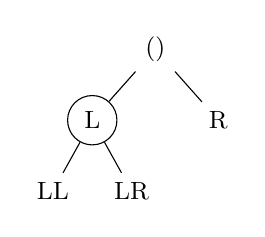
\begin{tikzpicture}[level distance=9mm,
        level 1/.style={sibling distance=16mm},
        level 2/.style={sibling distance=10mm},
        every node/.style={font=\small}]
      \node {$()$}
        child {node[circle, draw] {$\mathrm{L}$}
          child {node {$\mathrm{LL}$}}
          child {node {$\mathrm{LR}$}}}
        child {node {$\mathrm{R}$}};
    \end{tikzpicture}
    \hspace{2cm}
    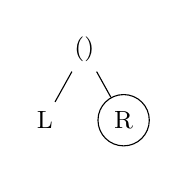
\begin{tikzpicture}[level distance=9mm,
        level 1/.style={sibling distance=10mm},
        every node/.style={font=\small}]
      \node {$()$}
        child {node {$\mathrm{L}$}}
        child {node[circle, draw] {$\mathrm{R}$}};
    \end{tikzpicture}

    \smallskip
    the tree $s$ \hspace{3.2cm} the subtree $s \dsub \mathrm{L}$
    \end{center}
\end{itemize}
Laws (D1)--(D5) are immediate.  The subtree at the root
is the whole tree, and concatenation of words is associative with the empty
word as unit.
\end{example}%
}}

\begin{theorem}\label{thm:main}
Every computable directed graph $G$ determines a computable directed
container $(V_G, P_G)$.
Fix $v \in V_G$ and $p \in P_G(v)$.  Then
\[
  \droot(v) = ()
  \qquad\text{and}\qquad
  v \dsub p = \mathrm{end}(p),
\]
and if $q \in P_G(v \dsub p)$ then
\[
  p \dshift q = pq \;\text{(concatenation)}.
\]
\end{theorem}

\begin{proof}
The container structure is a tautology --- we are just introducing
notation.  The computability content is small but real.  If $V$, $E$ are
computable sets and $\mathrm{src}$, $\mathrm{tgt}$ are computable maps
(Definition~\ref{def:comp-category}), then paths are finite sequences of
edge codes, and the three operations $\droot$ (the empty sequence),
$\dsub$ (read off the endpoint) and $\dshift$ (concatenate) are
computable maps on codes.
\end{proof}

\begin{remark}
Without concatenation we would not be able to turn the container into a
directed container.  The shift $\dshift$ requires composing two
positions, and the concatenation of an edge with an edge is not an
edge, but the concatenation of a path with a path is a path.  This is
the reason why we chose to make our positions paths rather than edges.
\end{remark}

\subsection{The computable case: coKleisli collapses to pure
functions}\label{sec:cokleisli-collapse}

What does the directed container structure buy us for computable
labellings (Section~\ref{sec:computations})?  Three things.

First, the laws of composition.  ``Sub-path = partial computation''
is meaningful because positions compose.  The fold satisfies
\[
  F(p \dshift q) = F(q) \circ F(p),
  \qquad
  F(\droot) = \mathrm{id},
\]
and these are exactly the directed container laws.

Second, the comonad runs the machine.  On a computable point
$\langle v, x_0 \rangle$ the counit $\varepsilon$ reads the current
value, and duplicate $\delta$ decorates every path $p$ out of $v$
with its intermediate state $\langle \mathrm{end}(p), \ell(p)
\rangle$: the entire tree of partial computations, unfolded from the
finite seed.  Comonad associativity says that restarting the
computation from any intermediate state agrees with the
straight-through run --- checkpointing is a law, not a hope.

Third, a collapse theorem.  In general a coKleisli map may inspect
the whole decorated context --- the entire history of the
computation.  On computable labellings the context is determined by
the current value, so every coKleisli map factors through
$\varepsilon$, and coKleisli composition reduces to ordinary
composition of functions.  Computable extensions form the
sub-coKleisli category on which
\[
  g \circ_{\mathrm{coK}} f = g \circ f.
\]
Hidden state is precisely the failure of a map to factor through
$\varepsilon$.

\begin{remark}
\label{rem:collision-witness}
The comonad gives an observable that detects non-computability.
Duplicate $\delta$ decorates each path $p$ with its shifted
sub-labelling $\ell_p = \ell(p \cdot -)$, the whole future from $p$.
The counit $\varepsilon$ reads only the present value $\ell(p)$.
Then
\[
  \ell \text{ is computable}
  \iff
  \ell_p \text{ is determined by } (\mathrm{end}(p), \ell(p)),
\]
i.e.\ $\delta$ carries no more information than $\varepsilon$.  A
violation is a \emph{collision witness}.  This is a triple $(p, q, r)$ with
\[
  \mathrm{end}(p) = \mathrm{end}(q),
  \qquad
  \ell(p) = \ell(q),
  \qquad
  \ell(p \cdot r) \neq \ell(q \cdot r).
\]
The present agrees but the futures diverge, so no edge functions can
generate $\ell$: the fold equation $f_e(\ell(p)) = \ell(p \cdot e)$
has no well-defined solution.

Every witness is finite data, so \emph{non}-computability is
semi-decidable.  Enumerate pairs of paths and continuations, and if
$\ell$ is not computable you will eventually find a witness.
Computability itself is never confirmed by finitely many
observations --- the next continuation could always break it.

In fact witnesses of length one suffice.  Paths of length $k$ are a
coproduct indexed by paths of length $k-1$,
\[
  P_k(v) \;\cong\; \sum_{p \in P_{k-1}(v)} E(\mathrm{end}(p)),
\]
--- a length-$k$ path is a length-$(k-1)$ path plus one outgoing edge
at its endpoint --- and $\mathrm{Path}(v) = \coprod_k P_k(v)$ grades
the path container by length.  Now take a collision witness
$(p, q, r)$ with $r = e_1 \cdots e_m$ minimal.  If $m > 1$ then
$\ell(p \cdot e_1) = \ell(q \cdot e_1)$ by minimality, so
$(p \cdot e_1,\, q \cdot e_1,\, e_2 \cdots e_m)$ is a shorter
witness.  Hence the minimal witness has $|r| = 1$: divergence, if it
happens at all, is visible one step after a value collision.

This gives a level-by-level algorithm.  Build level $k$ from level
$k-1$ via the coproduct.  Group the paths seen so far by the pair
$(\mathrm{end}(p), \ell(p))$.  Within each group check that the
one-step extensions agree.  So $\ell$ is computable if and only if
the partial function
\[
  (\mathrm{end}(p),\, \ell(p),\, e) \;\longmapsto\; \ell(p \cdot e)
\]
is well-defined --- the global fold property is equivalent to
one-step functionality.  If the graph and the value sets $X_v$ are
finite, there are at most $M = \sum_v |X_v|$ distinct pairs
$(\mathrm{end}(p), \ell(p))$, so checking paths of length up to $M$
decides computability outright.
\end{remark}

\begin{remark}
\label{rem:path-equivalence}
On a computable labelling, define $p \sim q$ when
$\mathrm{end}(p) = \mathrm{end}(q)$ and
$\ell(p \cdot r) = \ell(q \cdot r)$ for every continuation $r$.  In
the stateful picture proving $p \sim q$ required reasoning about
hidden machines.  Here it is two lines.  Taking $r$ to be the empty
path gives $\ell(p) = \ell(q)$.  Conversely, if
$\ell(p) = \ell(q)$ then for every $r$
\[
  \ell(p \cdot r) = F(r)(\ell(p)) = F(r)(\ell(q)) = \ell(q \cdot r),
\]
by the fold equation $F(p \cdot r) = F(r) \circ F(p)$.  So
\[
  p \sim q
  \iff
  \mathrm{end}(p) = \mathrm{end}(q)
  \;\text{ and }\;
  \ell(p) = \ell(q):
\]
behavioural equivalence collapses to equality of values.  The values
\emph{are} the states.  The quotient of paths by $\sim$ is the set of
reachable pairs $\langle \mathrm{end}(p), \ell(p) \rangle$ inside the
computable extension $\sum_{v} X_v$, which was the minimal machine
all along.
\end{remark}

\begin{remark}
\label{rem:partition-refinement}
The comonad gives an algorithm for finding the equivalence classes of
$\sim$.  Think of a labelling as a \emph{table}.  One row for each
path, holding its value.  Applying $\delta$ replaces each path by the
table of all paths extending it --- a table of tables.  Each inner
table starts at the vertex where its path ends, so the inner tables
sort into $n$ buckets, one per vertex.

Now iterate:
\begin{enumerate}
  \item Apply $\delta$: every path gets its table of continuations.
  \item Sort the inner tables into buckets by their start vertex.
  \item Within each bucket, group together the paths whose tables are
        equal (so far).
  \item Repeat one level deeper: groups that agreed to depth $k$ may
        split at depth $k+1$.
\end{enumerate}
When a round splits nothing, the partition has stabilised.

The resulting groups are the \emph{Myhill--Nerode classes}.  Two paths
lie in the same class when they end at the same vertex and their
tables agree on every continuation,
\[
  p \sim q
  \iff
  \mathrm{end}(p) = \mathrm{end}(q)
  \;\text{ and }\;
  \ell(p \cdot r) = \ell(q \cdot r) \text{ for all } r.
\]
The name comes from automata theory.  The states of the minimal
deterministic automaton recognising a language are exactly the
classes of words that no continuation can tell apart.  Here the same
idea applies with paths in place of words.  The classes at a vertex
$v$ are the genuinely distinguishable ways of arriving at $v$, and
their number is the amount of memory an implementation needs at $v$.

The outcome diagnoses the labelling:
\begin{itemize}
  \item one class per vertex: the future depends on the vertex alone.
  \item classes in bijection with the values $\ell(p)$: the values
        are the states, and the labelling is computable
        (Remark~\ref{rem:path-equivalence}).
  \item two classes sharing a value: a collision
        (Remark~\ref{rem:collision-witness}) --- the labelling needs
        hidden state beyond its values.
\end{itemize}
A discrepancy is a \emph{split}.  The two paths lie in different
classes.  Computable means the splitting stops --- finitely many
tables, forming a finite quotient graph on which the edges act as
functions.  At any finite stage we know neither.  Tables that agree
may split one level deeper, and the splitting may stop one level
later.  So we run for $M$ steps and judge.  If the graph and the
value sets are finite there are at most $\sum_v |X_v|$ classes, the
refinement stabilises, and the judgement becomes a proof.
\end{remark}

\section{Almost computable: Sturmian sequences}\label{sec:sturmian}

Since the refinement never delivers a verdict at a finite stage, we
grade the judgement.

\begin{definition}
\label{def:m-computable}
A labelling is \emph{$N$-not-computable} if a split occurs at
refinement step $N$, and \emph{$M$-computable} if the refinement runs
$M$ steps without a new split.  A labelling is computable if and only
if it is $N$-not-computable for only finitely many $N$.
\end{definition}

Splits never merge.  Refinement is monotone, so the sequence of
partitions converges to a limit partition --- the true Myhill--Nerode
classes.  Computable means the limit is reached at a finite step.
This also gives a distance on paths ending at the same vertex.  The
tables at $p$ and $q$ can be compared row by row, and we set
\[
  d(p,q) = 2^{-n}, \qquad
  n = \text{the length of the shortest continuation } r
      \text{ with } \ell(p \circ r) \neq \ell(q \circ r).
\]
The tables agree on all rows shorter than $n$ and first disagree at
depth $n$.  A disagreeing continuation of length $n$ is exactly a
split at refinement step $n$, so this is the same number counted two
ways.  Equivalence, $p \sim q$, means the tables agree at every
depth: $d(p,q) = 0$.  The distance is an ultrametric ---
$d(p,q) \leq \max(d(p,r), d(r,q))$, since tables that each agree with
a third to depth $n$ agree with each other to depth $n$ --- and the
classes at step $n$ are the balls of radius $2^{-n}$.

How slowly can a labelling fail to be computable?  Take the simplest
graph.  It has one vertex $u$ and one loop $a$.  There is exactly one path
$a^k$ of each length, all ending at $u$, so a labelling is an
infinite sequence $\ell_k = \ell(a^k)$, and the refinement partitions
the set of \emph{all} paths $\{a^0, a^1, a^2, \dots\}$ at once.

To compare two paths $p = a^j$ and $q = a^k$ we compare their values
on extensions: $\ell(p \circ r)$ against $\ell(q \circ r)$ for
$r = a, a^2, a^3, \dots$.  Refinement step $n$ checks the extensions
of length $n$.  So $p$ and $q$ lie in the same class at step $n$
exactly when they agree on all extensions of length at most $n$
(including the empty one, their own values):
\[
  \ell_{j+m} = \ell_{k+m} \quad \text{for } m = 0, 1, \dots, n,
\]
that is, when the sequence looks the same for $n+1$ terms from
position $j$ as from position $k$.  A class at step $n$ is therefore
a \emph{window} of length $n+1$ --- each path $a^k$ carries the
window starting at position $k$, and two paths are in the same class
when they carry the same window.  The number of classes at step $n$
is the number of \emph{distinct} windows of length $n+1$ occurring
in the sequence.  This is the \emph{factor complexity} $p(n+1)$.

A split is now concrete.  Passing from step $n$ to step $n+1$
extends each window by one letter.  Most windows $w$ extend in only
one way --- every occurrence of $w$ in the sequence is followed by
the same letter --- and those classes survive intact.  A window $w$
that occurs somewhere followed by $0$ and somewhere else followed by
$1$ splits into two classes, $w0$ and $w1$.

The theorem of Morse and Hedlund \cite{morsehedlund} says a sequence
is eventually periodic if and only if $p$ is bounded --- our
computable case, a finite quotient graph --- and otherwise
$p(n) \geq n+1$.  A \emph{Sturmian sequence}
\cite{morsehedlund2} attains the minimum: $p(n) = n+1$, exactly
one split per level, forever.  Sturmian labellings are
$N$-not-computable for every $N$, but as slowly as possible.  They are
the almost computable labellings.  The standard example is an
irrational rotation, $\ell_k = \lfloor (k+1)\alpha \rfloor - \lfloor
k\alpha \rfloor$ for irrational $\alpha$.  For $\alpha = 1/\varphi^2$
this is the Fibonacci word.

There is a phase transition.  Morse--Hedlund is a \emph{gap}
theorem.  Either $c(n)$ is bounded or $c(n) \geq n+2$ --- no
labelling splits logarithmically often, and no labelling fails to be
computable more slowly than one split per step.  Above the gap the
spectrum is continuous:
\begin{itemize}
  \item \emph{bounded}: eventually periodic sequences --- the
        computable labellings, finite quotient graphs.
  \item \emph{linear}, $c(n) = n+2$: Sturmian sequences, the
        irrational rotations --- one split per step, almost
        computable.
  \item \emph{polynomial}: for example billiard words in higher
        dimensions, with quadratic complexity.
  \item \emph{exponential}, $c(n) = 2^{n+1}$: random sequences ---
        every class splits at every step, maximally not computable.
\end{itemize}
Computability has a hard edge --- it is left at speed exactly one
split per step, never slower --- while non-computability is graded
all the way up to $2^{n+1}$.

The class counts assemble into a generating function
$C(x) = \sum_n c(n)\, x^n$, and the phase transition becomes a
statement about its coefficients:
\begin{itemize}
  \item computable: bounded coefficients, $C(x)$ rational with a
        simple pole at $x = 1$.
  \item Sturmian: $c(n) = n+2$, a double pole at $x = 1$,
        \[
          C(x) = \frac{2 - x}{(1-x)^2}.
        \]
  \item random: $c(n) = 2^{n+1}$, pole at $x = \tfrac12$.
\end{itemize}
The Morse--Hedlund gap says the pole at $x = 1$ has order $1$ or at
least $2$ --- the coefficients cannot grow like $\log n$ or
$\sqrt{n}$.  For substitutive words such as Fibonacci and Pell the
complexity generating function is rational.  The finite generating
rule appears as rationality of the coefficient series.
Computability of a labelling is rationality, with pole only at
$x = 1$ and order $1$, of its class-count series.

\subsection{Experiment}\label{sec:refinement-experiment}

\paragraph{Setup.}
The graph is one vertex $u$ with one loop $a$, the value set is
$X_u = \texttt{Bool}$, and a labelling is an infinite bit sequence
$\ell_k = \ell(a^k)$.  We compare two labellings:
\begin{itemize}
  \item \emph{Fibonacci}: the Sturmian word generated by the
        substitution $0 \mapsto 01$, $1 \mapsto 0$, iterated from
        $0$.  Equivalently it is the rotation
        $\ell_k = \lfloor (k+1)\alpha \rfloor - \lfloor k\alpha
        \rfloor$ with $\alpha = 1/\varphi^2$.  It begins
        $0100101001001\dots$
  \item \emph{Random}: independent uniform bits from a seeded
        pseudorandom generator.
\end{itemize}
Each word is truncated to its first $L = 10^5$ letters.

\paragraph{Method.}
On this graph the refinement collapses to window counting.  The
table at the path $a^k$ is the tail $(\ell_k, \ell_{k+1}, \dots)$,
and two paths lie in the same class after $n$ refinement steps
exactly when their tails agree for $n+1$ terms.  So the class count
at step $n$ is
\[
  c(n) \;=\; \#\{\, (\ell_i, \dots, \ell_{i+n}) : i \geq 0 \,\}
  \;=\; p(n+1),
\]
the number of distinct windows of length $n+1$.  The program slides
a window of length $n+1$ along the word, collects the windows into a
set, and reports its size, for $n = 0, \dots, 25$.  A \emph{split}
at step $n$ is an increase $c(n) > c(n-1)$: the class of a window
$w$ splits when both $w0$ and $w1$ occur.

\paragraph{Results.}
\[
\begin{array}{r|cccccccc|cccc}
  \text{step } n & 0 & 1 & 2 & 3 & 4 & 5 & 6 & 7
                 & 13 & 17 & 21 & 25 \\
  \hline
  \text{Fibonacci} & 2 & 3 & 4 & 5 & 6 & 7 & 8 & 9
                   & 15 & 19 & 23 & 27 \\
  \text{random}    & 2 & 4 & 8 & 16 & 32 & 64 & 128 & 256
                   & 16328 & 83031 & 98799 & 99906
\end{array}
\]

The Fibonacci word splits exactly once per step at every one of the
$25$ steps: $c(n) = n+2$, the Morse--Hedlund minimum for an
aperiodic word.  In the ultrametric, each step shaves one ball off
one class and leaves every other class untouched.  The labelling is
$N$-not-computable for every $N$, but a single counter of splits
suffices to describe its failure.

The random word splits everywhere.  Every class splits in two at
every step, $c(n) = 2^{n+1}$, the maximal possible rate --- every
window of every length occurs.  The balls halve at every level, so
the completion of the path space is the full Cantor set
$2^{\mathbb{N}}$.  Linear against exponential growth of $c(n)$ is
the measured difference between \emph{barely} not computable and
\emph{maximally} not computable.

\paragraph{The data horizon.}
The doubling holds only through step $13$.  From there the random
counts bend --- $16328$, $31096$, $51090$, \dots, $99906$ ---
approaching the ceiling $L - n$: a word of length $10^5$ contains at
most $10^5 - n$ windows of length $n+1$, and fewer than $2^{n+1}$
once $n > \log_2 L \approx 17$.  The splitting has not slowed.  The
sample has run out of witnesses.  This is the judgement at $M$ steps
in its strictest form.  Beyond the data horizon the experiment cannot
even see the splits, and the Fibonacci column --- which marches on
at one split per step, unbothered by the horizon --- is the only one
whose observed counts still equal the true ones.

\paragraph{Coefficients of power series.}
Working over $\mathbb{N}$ trivialises the question.  If the
coefficients are all distinct (Catalan, factorials, $2^n$) then
$f(a_k) = a_{k+1}$ is a well-defined function on the value set, the
value is the state, and the labelling is computable with no splits
at all.  To force collisions we reduce mod $2$ and label the paths
$a^k$ with the $k$-th coefficient in $\mathbb{F}_2$.  By Christol's
theorem \cite{christol}, the coefficient sequence of a power series
over $\mathbb{F}_2$ is $2$-automatic if and only if the series is
algebraic over $\mathbb{F}_2(x)$.  Automatic sequences have factor
complexity $O(n)$ \cite{cobham, alloucheshallit}.  We ran the
refinement on the first
$2 \times 10^5$ coefficients of three series, one from each analytic
class:

\[
\begin{array}{r|ccccccc|cc}
  \text{step } n & 0 & 1 & 2 & 3 & 4 & 5 & 6 & 14 & 22 \\
  \hline
  \text{Fibonacci numbers mod } 2 & 2 & 3 & 3 & 3 & 3 & 3 & 3 & 3 & 3 \\
  \text{Catalan numbers mod } 2   & 2 & 4 & 6 & 7 & 9 & 11 & 12 & 24 & 39 \\
  \text{partition numbers mod } 2 & 2 & 4 & 8 & 16 & 32 & 64 & 128
    & 32698 & 197513
\end{array}
\]

The analytic trichotomy of the generating function is read off from
the splitting rate of its coefficient labelling:
\begin{itemize}
  \item \emph{rational} (Fibonacci numbers, period $011$ mod $2$):
        the splitting stops at $3$ classes --- computable, the
        quotient is a $3$-cycle.
  \item \emph{algebraic} (Catalan numbers, odd exactly at
        $n = 2^k - 1$): one or two splits per step --- the automatic
        band, linear like Sturmian, almost computable.
  \item \emph{transcendental?} (partition numbers): every class
        splits at every step, $c(n) = 2^{n+1}$ up to the data
        horizon --- indistinguishable from random.  The refinement
        cannot tell $p(n) \bmod 2$ from coin flips, consistent with
        the conjecture that partition parity is normal.
\end{itemize}
Nothing in the algorithm knows about power series --- it only
compares futures of paths --- yet the splitting rate recovers the
rational/algebraic/transcendental classification of the generating
function.

On the one-loop graph our refinement specialises to factor
complexity, and the results above are classical
\cite{morsehedlund, cobham, christol}.  The contribution here is
the comonadic formulation.  The refinement is generated by $\delta$,
it makes sense on any coloured graph, and there the paths arriving
at each vertex form a family of ultrametric spaces about which,
as far as we know, nothing is known.

\section{Application: a toy knowledge graph}\label{sec:knowledge-graph}

We build a toy knowledge graph.  The vertices are
\[
  V = \{\textsf{author}, \textsf{paper}, \textsf{definition},
        \textsf{theorem}, \textsf{example}\},
\]
and the edges are the relations
\begin{itemize}
  \item $\textsf{wrote} : \textsf{author} \to \textsf{paper}$,
  \item $\textsf{includes} : \textsf{paper} \to \textsf{definition}$,
        $\textsf{paper} \to \textsf{theorem}$,
        $\textsf{paper} \to \textsf{example}$,
  \item $\textsf{uses} : \textsf{theorem} \to \textsf{definition}$,
        $\textsf{theorem} \to \textsf{theorem}$,
  \item $\textsf{exampleOf} : \textsf{example} \to \textsf{definition}$,
  \item $\textsf{specialCaseOf} : \textsf{theorem} \to \textsf{theorem}$,
  \item $\textsf{proves} : \textsf{theorem} \to \textsf{theorem}$.
\end{itemize}
Note the three loops at $\textsf{theorem}$: a theorem may use, prove,
or be a special case of, another theorem.

\appendix

\section{Containers are distributive}\label{app:distributive}

Recall that a container morphism $(u, g) : \psi \to \varphi$ has
$u$ \emph{forwards} on shapes and $g$ \emph{backwards} on positions
($g_s : \hat{P}(u(s)) \to P(s)$).  This contravariance decides
everything below.

\emph{The sum is the coproduct.}  A morphism \emph{out of}
$\psi + \varphi$ into some container $\chi$ consists of a map out
of $S \sqcup \hat{S}$ --- which, by the universal property of the
disjoint union, is exactly a case split into a map out of $S$ and a map
out of $\hat{S}$ --- together with backwards position arrows landing
in $(P \sqcup \hat{P})(s)$, which is $P(s)$ or $\hat{P}(s)$
according to the side.  So a morphism $\psi + \varphi \to \chi$
is exactly a pair of morphisms $\psi \to \chi$ and
$\varphi \to \chi$, naturally.  The universal property of the
coproduct.

\emph{The product is the product.}  A morphism \emph{into}
$\psi \times \varphi$ from some container $\chi = (R, Q)$
consists of a map $R \to S \times \hat{S}$ --- a \emph{pairing},
by the universal property of the cartesian product --- together
with backwards position arrows
$P(s) \sqcup \hat{P}(\hat{s}) \to Q(r)$.  A map \emph{out of} a
disjoint union is again a case split, i.e.\ a pair of maps
$P(s) \to Q(r)$ and $\hat{P}(\hat{s}) \to Q(r)$.  So a morphism
$\chi \to \psi \times \varphi$ is exactly a pair of morphisms
$\chi \to \psi$ and $\chi \to \varphi$: the universal property
of the product.  Note how the contravariance of positions flips
the coproduct of position sets into what the \emph{product} of
containers requires --- this is why the product of containers
takes the \emph{disjoint union} of positions.

\emph{Distributivity.}  Write $\psi = (S, P)$,
$\varphi_i = (T_i, Q_i)$.  Compare the two sides of the canonical
map:
\begin{itemize}
  \item shapes: $(S \times T_1) \sqcup (S \times T_2)$ on the left,
    $S \times (T_1 \sqcup T_2)$ on the right.  The canonical map
    between them is precisely the distributivity isomorphism of
    \emph{sets} --- the pair $(s, \text{``$t_1$ or $t_2$''})$ is
    the same data as ``$(s, t_1)$ or $(s, t_2)$''.
  \item positions: at a shape $(s, t)$ with $t$ on side $i$,
    \emph{both} containers assign $P(s) \sqcup Q_i(t)$, and the
    canonical map is the identity.
\end{itemize}
An isomorphism on shapes together with the identity on positions is
an isomorphism of containers, so the canonical map is invertible
and the category of containers is distributive.  All the
distributivity lives in the shapes and is inherited from
$\mathbf{Set}$.  The positions just come along for the ride.
(Alternatively, the extension $\psi \mapsto C_\psi$ embeds
containers fully faithfully into functors, turns container sum and
product into \emph{pointwise} sum and product
(Remark~\ref{rem:extension-is-sum}), and pointwise operations
distribute because $\mathbf{Set}$ does.  A fully faithful functor
reflects isomorphisms.)

\section{Proof of Exercise~\ref{ex:kleisli-monad}: Kleisli maps make
a monad}\label{app:kleisli}

Suppose $T$ admits Kleisli maps.  Unpacking ``$g \bullet f =
g^\dagger \circ f$ is associative with unit $\eta$'' gives three
laws:
\begin{itemize}
  \item[(K1)] $\eta_X^\dagger = \mathrm{id}_{T(X)}$
    \hfill ($\eta$ is a left unit: $f \bullet \eta \dots$ read at
    $f = \mathrm{id}$),
  \item[(K2)] $f^\dagger \circ \eta_X = f$
    \hfill ($\eta$ is a right unit: $f \bullet \eta = f$),
  \item[(K3)] $(g^\dagger \circ f)^\dagger = g^\dagger \circ
    f^\dagger$
    \hfill (associativity: $(h \bullet g) \bullet f = h \bullet (g
    \bullet f)$).
\end{itemize}
This data is a \emph{Kleisli triple}.  From it we build a monad:
\[
  T(f) = (\eta_Y \circ f)^\dagger \quad (f : X \to Y),
  \qquad
  \mu_X = (\mathrm{id}_{T(X)})^\dagger : T(T(X)) \to T(X).
\]
The functor laws:
$T(\mathrm{id}) = \eta^\dagger = \mathrm{id}$ by (K1), and
\[
  T(g) \circ T(f)
  = (\eta g)^\dagger (\eta f)^\dagger
  \overset{\text{(K3)}}{=} \bigl((\eta g)^\dagger \eta f\bigr)^\dagger
  \overset{\text{(K2)}}{=} (\eta g f)^\dagger
  = T(g f).
\]
The monad laws:
\[
  \mu \circ \eta = \mathrm{id}^\dagger \circ \eta
    \overset{\text{(K2)}}{=} \mathrm{id},
  \qquad
  \mu \circ T(\eta) = \mathrm{id}^\dagger (\eta\eta)^\dagger
    \overset{\text{(K3)}}{=} (\mathrm{id}^\dagger \eta \eta)^\dagger
    \overset{\text{(K2)}}{=} \eta^\dagger
    \overset{\text{(K1)}}{=} \mathrm{id},
\]
\[
  \mu \circ \mu
  = \mathrm{id}^\dagger \mathrm{id}^\dagger
  \overset{\text{(K3)}}{=} (\mathrm{id}^\dagger \mathrm{id})^\dagger
  = (\mathrm{id}^\dagger)^\dagger
  \overset{\text{(K2)}}{=} \bigl(\mathrm{id}^\dagger (\eta\,
    \mathrm{id}^\dagger)\bigr)^\dagger
  \overset{\text{(K3)}}{=} \mathrm{id}^\dagger (\eta\,
    \mathrm{id}^\dagger)^\dagger
  = \mu \circ T(\mu),
\]
and naturality of $\eta$ and $\mu$ are similar (K2)/(K3)
manipulations.

Conversely, a monad $(T, \eta, \mu)$ admits Kleisli maps.  Set
$f^\dagger = \mu_Y \circ T(f)$.  Then (K1) is the unit law
$\mu \circ T(\eta) = \mathrm{id}$, (K2) is naturality of $\eta$
followed by $\mu \circ \eta = \mathrm{id}$, and (K3) is naturality
of $\mu$ followed by associativity $\mu \circ T(\mu) = \mu \circ
\mu$.  So ``being a monad'' and ``admitting Kleisli maps'' are the
same structure presented differently.  A monad is exactly what it
takes for the effectful maps $X \to T(Y)$ to form a category.

\section{Proof of Exercise~\ref{ex:cokleisli-directed}: coKleisli
maps make a directed container}\label{app:cokleisli}

Dualise Appendix~\ref{app:kleisli}.  ``$g \bullet f = g \circ
\mathrm{extend}(f)$ is associative with unit $\varepsilon$'' unpacks
to the dual laws:
\begin{itemize}
  \item[(C1)] $\mathrm{extend}(\varepsilon_X) = \mathrm{id}_{W(X)}$,
  \item[(C2)] $\varepsilon_Y \circ \mathrm{extend}(f) = f$,
  \item[(C3)] $\mathrm{extend}(g \circ \mathrm{extend}(f)) =
    \mathrm{extend}(g) \circ \mathrm{extend}(f)$,
\end{itemize}
a \emph{coKleisli triple} on $W$.  Equivalently it is a comonad, with
$\delta_X = \mathrm{extend}(\mathrm{id}_{W(X)}) : W(X) \to W(W(X))$.
What remains is specific to containers.  To show that a coKleisli
triple on the \emph{extension of a container}, acting on labellings
and leaving shapes alone, is the same thing as directed-container
structure $(\droot, \dsub, \dshift)$ on $\psi$ satisfying D1--D5.
This is the theorem of Ahman--Chapman--Uustalu \cite{acu}.  We give
the dictionary.

\emph{From operations to structure.}  Given a directed container,
define
\[
  \varepsilon\langle s, f \rangle = f(\droot(s)),
  \qquad
  \mathrm{extend}(f)\langle s, h \rangle =
  \langle s,\; p \mapsto f\langle s \dsub p,\;
    q \mapsto h(p \dshift q)\rangle\rangle.
\]

\emph{From structure to operations.}  Conversely, given
$\varepsilon$ and $\mathrm{extend}$, apply them to \emph{generic}
elements.  Take $X = P(s)$ and the identity labelling, giving
$w_s = \langle s, \mathrm{id}_{P(s)} \rangle \in W(P(s))$.  Then:
\[
  \droot(s) = \varepsilon(w_s) \in P(s),
\]
and $\delta(w_s) = \langle s,\; p \mapsto \langle \sigma(p),
k_p \rangle \rangle$ for some shapes $\sigma(p)$ and labellings
$k_p : P(\sigma(p)) \to P(s)$.  Read off
\[
  s \dsub p = \sigma(p),
  \qquad
  p \dshift q = k_p(q).
\]

\emph{The laws.}  Writing $\delta\langle s, f\rangle = \langle s,\;
p \mapsto \langle s \dsub p,\; q \mapsto f(p \dshift q)
\rangle\rangle$, the two counit laws and coassociativity translate
exactly into D1--D5:
\begin{itemize}
  \item $\varepsilon \circ \delta = \mathrm{id}$: compute
    $\varepsilon(\delta\langle s, f\rangle) =
    \langle s \dsub \droot(s),\; q \mapsto f(\droot(s) \dshift q)
    \rangle$.  Equality with $\langle s, f \rangle$ forces
    \[
      s \dsub \droot(s) = s \;\;(\mathrm{D1}),
      \qquad
      \droot(s) \dshift q = q \;\;(\mathrm{D2}).
    \]
  \item $W(\varepsilon) \circ \delta = \mathrm{id}$: compute
    $W(\varepsilon)(\delta\langle s, f\rangle) = \langle s,\;
    p \mapsto f(p \dshift \droot(s \dsub p))\rangle$.  Equality
    with $\langle s, f \rangle$ forces
    \[
      p \dshift \droot(s \dsub p) = p \;\;(\mathrm{D3}).
    \]
  \item $\delta$ coassociative, $(W\delta) \circ \delta =
    (\delta W) \circ \delta$: both sides are labellings of
    labellings of labellings.  Comparing the shape components forces
    \[
      s \dsub (p \dshift q) = (s \dsub p) \dsub q \;\;(\mathrm{D4}),
    \]
    and comparing the position components forces
    \[
      (p \dshift q) \dshift r = p \dshift (q \dshift r)
      \;\;(\mathrm{D5}).
    \]
\end{itemize}
So the five directed-container laws are not axioms imposed from
outside.  They are precisely the statement that context-dependent
maps $W(X) \to Y$ compose associatively with ``evaluate here'' as
the identity.  A directed container is exactly what it takes for
observations-in-context to form a category --- dually to
Appendix~\ref{app:kleisli}, where a monad is exactly what it takes
for effectful maps to do so.

\begin{thebibliography}{9}
\bibitem{acg}
M.~Abbott, T.~Altenkirk, and N.~Ghani.
\newblock Containers: Constructing strictly positive types.
\newblock \emph{Theoretical Computer Science}, 342:3--27, 2005.

\bibitem{acu}
D.~Ahman, J.~Chapman, and T.~Uustalu.
\newblock When is a container a comonad?
\newblock In \emph{FoSSaCS}, LNCS 7213, 2012.

\bibitem{au16}
D.~Ahman and T.~Uustalu.
\newblock Directed containers as categories.
\newblock \emph{EPTCS}, 207:89--98, 2016.

\bibitem{langer2026}
R.~Langer.
\newblock Directed containers in trust boundaries: How proof registries are
  comonads.
\newblock 2026.

\bibitem{morsehedlund}
M.~Morse and G.~A.~Hedlund.
\newblock Symbolic dynamics.
\newblock \emph{American Journal of Mathematics}, 60(4):815--866, 1938.

\bibitem{morsehedlund2}
M.~Morse and G.~A.~Hedlund.
\newblock Symbolic dynamics II: Sturmian trajectories.
\newblock \emph{American Journal of Mathematics}, 62(1):1--42, 1940.

\bibitem{cobham}
A.~Cobham.
\newblock Uniform tag sequences.
\newblock \emph{Mathematical Systems Theory}, 6:164--192, 1972.

\bibitem{christol}
G.~Christol, T.~Kamae, M.~Mend\`es France, and G.~Rauzy.
\newblock Suites alg\'ebriques, automates et substitutions.
\newblock \emph{Bulletin de la Soci\'et\'e Math\'ematique de France},
  108:401--419, 1980.

\bibitem{alloucheshallit}
J.-P.~Allouche and J.~Shallit.
\newblock \emph{Automatic Sequences: Theory, Applications,
  Generalizations}.
\newblock Cambridge University Press, 2003.
\end{thebibliography}

\end{document}
